\section{Réfraction de la lumière}

\begin{figure}
\centering
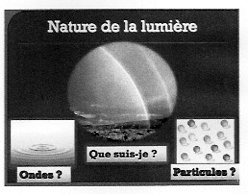
\includegraphics[width=5.366cm,height=4.175cm]{Pictures/10000001000000F8000000C2693C9AC6103FFED7.png}
\caption{}
\end{figure}

L'expérience de Young nous a permis d'affirmer que la lumière a un
comportement ondulatoire.

Continuons la démarche dans le cadre de la dualité onde-particule de la
lumière, et intéressons-nous à la réfraction de la lumière. Cette
dernière obéit-elle à la loi de Snell~élaborée avec la cuve à onde,
autrement dit, la lumière a-t-elle un comportement ondulatoire si elle
est soumise au phénomène de la réfraction~?

La question que nous nous posons est de savoir si la lumière obéit à la
loi de Snell.

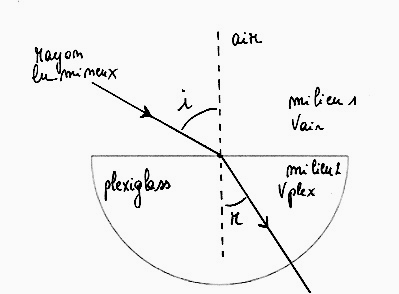
\includegraphics[width=7.398cm,height=5.456cm]{Pictures/100000010000018F0000012698B477377A07703C.png}\emph{Expérience~:
}

Pour ce faire, faisons réfracter la lumière monochromatique à travers un
prisme semi-circulaire en plexiglas et observons la relation entre
l'angle d'incidence, l'angle de réfraction, la vitesse de la lumière
dans l'air (v\textsubscript{1}) et la vitesse de la lumière dans le
plexiglas (v\textsubscript{2}).

\subsection{Observations }

Lorsqu'un rayon lumineux passe de l'air au plexiglas, nous pouvons
observer que $\theta_r$ (le rayon se rapproche de la normale).

Il nous reste à savoir si $v_{1} > v_{2}$ ,
autrement dit, si la vitesse de la lumière dans l'air est supérieure à la vitesse
de la lumière dans le plexiglas.

Comment faire~? La vitesse de la lumière est de l'ordre de 300 000
km/s~!!! C'est impossible de la mesurer dans notre petit laboratoire
terrestre \ldots.

\begin{figure}
\centering

\includegraphics[width=1.898cm,height=2.048cm]{Pictures/1000000100000184000001A368D3CEB0029E7460.png}
\caption{}
\end{figure}

Nous pouvons calculer le rapport des vitesses car nous savons déterminer
le rapport des longueurs d'onde grâce à l'expérience de diffraction de
la lumière par un réseau~!!!!

Ceci fera l'objet du laboratoire suivant. Nous reviendrons à nos moutons
ensuite, lorsque nous aurons déterminé si la lumière se propage plus
rapidement dans l'air que dans l'eau ( ou le plexiglas) ou inversement.

\subsection{Laboratoire - Détermination du rapport des vitesses de la lumière dans l'air et dans l'eau}

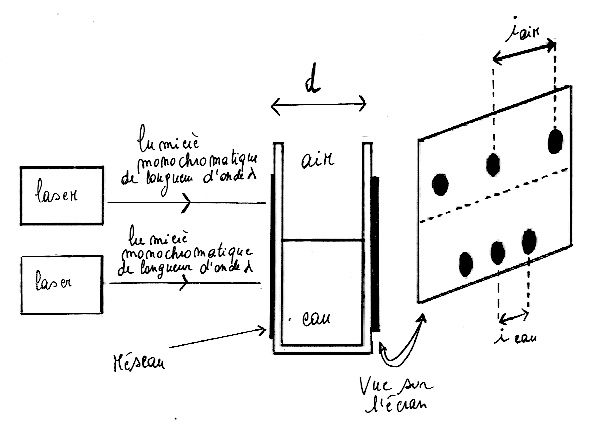
\includegraphics[width=9.885cm,height=7.243cm]{Pictures/1000000100000257000001B74156330002E2CF55.png}

\paragraph{Dispositif expérimental}

On utilise de la lumière monochromatique (une seule fréquence) d'un
laser.

Un réseau de 530 traits par mm est placé contre une des faces du
réservoir rempli en partie d'eau.

L'écran est placé contre la face opposée à celle où est placé le réseau.

La hauteur du laser sera ajustée pour que la lumière traverse tantôt de
l'air, tantôt de l'eau.

En mesurant i\textsubscript{air} et i\textsubscript{eau }, nous pouvons
calculer expérimentalement le rapport des vitesses de la lumière dans
l'air et dans l'eau (vair/veau).

Mesures expérimentales~:
\begin{enumerate}
	\item Mesure de $i$ dans l'air~:
	\item Mesure de $i$ dans l'eau~:
	\item Calculer le rapport $\frac{v_\text{air}}{v_\text{eau}}} $ sachant
que $ V= ??$ 

\end{enumerate}


Conclusion~: La lumière se propage plus rapidement dans l'air que dans
l'eau.

La diffraction de la lumière par un réseau conduit à la
conclusion que la lumière se propage plus rapidement dans l'air que dans
l'eau.

\subsection{Réfraction de la lumière allant de l'air dans le plexiglas (ou dans l'eau)}

Grâce au laboratoire précédent, nous avons
expérimentalement déterminé que \emph{la vitesse de la lumière dans
l'air est supérieure à la vitesse de la lumière dans l'eau} (ou dans le
plexiglas)}{Grâce au laboratoire précédent, nous avons expérimentalement déterminé que la vitesse de la lumière dans l'air est supérieure à la vitesse de la lumière dans l'eau (ou dans le plexiglas)

La question que nous nous posons est de savoir si la lumière obéit à la
loi de Snell.

Pour ce faire, revenons à nos moutons et faisons réfracter la lumière
monochromatique à travers un prisme semi-circulaire en plexiglas et
observons la relation entre l'angle d'incidence, l'angle de réfraction,
la vitesse de la lumière dans l'air et la vitesse de la lumière dans le
plexiglas.

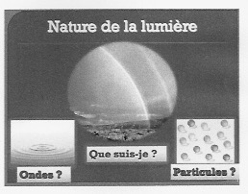
\includegraphics[width=6.172cm,height=4.551cm]{Pictures/10000001000000F8000000C25D3572F9FC1A2068.png}

Grâce à l'expérience de Young, réalisée dans l'air et dans le plexiglas (comme
nous l'avions réalisée dans l'air et dans l'eau), nous pouvons
expérimentalement déterminer que~\emph{pour la lumière }:
$ v_\mbox{air} > v_mbox{plexi} $

Et nous avons observé expérimentalement (voir figure ci-contre)~:
$\theta_i < \theta_r$ FIXME à vérifier

\begin{figure}
\centering
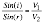
\includegraphics[width=2.634cm,height=1.412cm]{Pictures/100000010000002B00000017F74A96A4365CCDCA.png}
\caption{}
\end{figure}

et donc~:

\begin{figure}
\centering
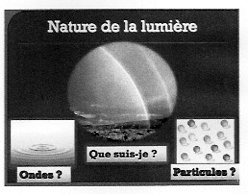
\includegraphics[width=5.366cm,height=4.175cm]{Pictures/10000001000000F8000000C2693C9AC6103FFED7.png}
\caption{}
\end{figure}

\emph{\textbf{3. Conclusion quand au caractère ondulatoire ou
corpusculaire de la lumière }}

LUMIERE~: ONDE OU PARTICULE~?

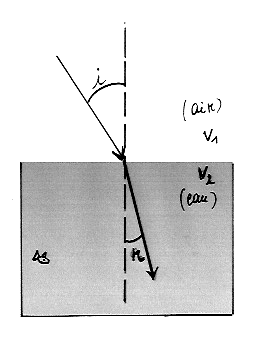
\includegraphics[width=3.829cm,height=4.334cm]{Pictures/1000000100000102000001673F5D940D6E4D1166.png}1)
Si nous nous reportons à l'expérience de réfraction avec la lumière~:

Lorsque la lumière passe de l'air à l'eau, nous observons de la
réfraction avec~:

i  r

et v\textsubscript{air}  v\textsubscript{eau}
(v\textsubscript{1}v\textsubscript{2})

Ce qui est conforme à la loi de Snell (ondulatoire).

Cela confère à la lumière un \emph{comportement ondulatoire.}

2) Les phénomènes de diffraction et d'interférences ne sont explicables
que par un comportement ondulatoire. Or la lumière diffracte et est
soumise aux interférences. Elle a donc un \emph{comportement
ondulatoire.}

3) La diffraction de la lumière par un réseau conduit à la conclusion
que la lumière se propage plus rapidement dans l'air que dans l'eau.

Cela lui confère un \emph{comportement corpusculaire.}

4) La propagation de la lumière dans le vide (donc en l'absence de
milieu), lui confère un \emph{comportement corpusculaire.}

Nous ne sommes pas sortis de l'auberge \ldots.

Cette dualité prend ses racines dans un
\href{https://www.techno-science.net/definition/4206.html}{\emph{\emph{débat}}}
remontant aussi loin que le XVII\textsuperscript{e}~siècle , quand
s'affrontaient les théories concurrentes de Christiaan Huygens qui
considérait que la
\href{https://www.techno-science.net/glossaire-definition/Lumiere.html}{\emph{\emph{lumière}}}
était composée d'ondes et celle de
\href{https://www.techno-science.net/glossaire-definition/Isaac-Newton.html}{\emph{\emph{Isaac
Newton}}} qui considérait que la lumière était des particules.

En attendant de continuer cette démarche scientifique qui permettrait de
trouver une réponse à cette dualité, nous allons nous attarder à
exploiter les expériences et théories relatives à la réfraction de la
lumière et à sa diffraction par un réseau.

Passons aux exercices et applications au chapitre suivant.
